\documentclass{article}
\usepackage[margin=0.5in]{geometry}
\usepackage{amsfonts}
\usepackage{amsmath}
\usepackage{graphicx}
\graphicspath{ {./pictures/} }


\author{Aaron Hao Tan}
\title{Reinforcement Learning Equations}
\date{\vspace{-5ex}}

\begin{document}
\maketitle

\noindent
\section{Finite Markov Decision Processes}

\noindent
\textbf{Components of MDP}
: {Decision epochs, State, Action, Transition probability,
Rewards}
\begin{equation}
\left\{T, S, A_{s}, p_{t}(\cdot | s, a), r_{t}(s, a)\right\}
\end{equation}

\noindent
A state is \textit{Markov} if and only if 

\begin{equation}
\mathbb{P}\left[S_{t+1} | S_{t}\right]=\mathbb{P}\left[S_{t+1} | S_{1}, \ldots, S_{t}\right]
\end{equation}

\noindent
\textbf{State-transition probabilities}
($p$ characterize the environment's dynamics).
More often used than equations 4 and 5.

\begin{equation}
\begin{aligned}
p(s^{\prime} | s, a) &= Pr [S_{t} = s^{\prime} | S_{t-1}=s, A_{t-1}=a] \\
&=\sum_{r \in \mathcal{R}} p(s^{\prime}, r | s, a)
\end{aligned}
\end{equation}

\noindent
\textbf{Expected rewards }
for state-action pairs and for state-action-next-state triples.
The current reward depends on the previous state and action.

\begin{equation}
r(s, a) \doteq \mathbb{E} \left[R_{t} | S_{t-1}=s, A_{t-1}=a\right]=\sum_{r \in \mathcal{R}} r \sum_{s^{\prime} \in \mathcal{S}} p\left(s^{\prime}, r | s, a\right)
\end{equation}

\begin{equation}
r\left(s, a, s^{\prime}\right) \doteq \mathbb{E}\left[R_{t} | S_{t-1}=s, A_{t-1}=a, S_{t}=s^{\prime}\right]=\sum_{r \in \mathcal{R}} r \frac{p\left(s^{\prime}, r | s, a\right)}{p\left(s^{\prime} | s, a\right)}
\end{equation}

\noindent
\textbf{Policy }
\\
- Probabilistic is inferior to deterministic

\begin{equation}
\pi(a | s)= Pr(A_{t} = a | S_{t}=s)
\end{equation}

\noindent
\textbf{Returns (sum of rewards) }
\begin{equation}
G_{t} \doteq R_{t+1}+R_{t+2}+R_{t+3}+\cdots+R_{T}
\end{equation}

\noindent
\textbf{Discounted Returns }
($\gamma$ = discount rate). If $\gamma < 1$, the infinite sum
in equation 8 would have a finite value. If $\gamma = 0$, the agent is concerned
with only maximizing immediate rewards (myopic). If the reward is +1, the return
is equivalent to $G_{t}=\sum_{k=0}^{\infty} \gamma^{k}=\frac{1}{1-\gamma}$.
\begin{equation}
G_{t} \doteq R_{t+1}+\gamma R_{t+2}+\gamma^{2} R_{t+3}+\cdots=\sum_{k=0}^{\infty} \gamma^{k} R_{t+k+1}
\end{equation}
\begin{equation}
\begin{aligned}
G_{t} & \doteq R_{t+1}+\gamma R_{t+2}+\gamma^{2} R_{t+3}+\gamma^{3} R_{t+4}+\cdots \\
&=R_{t+1}+\gamma\left(R_{t+2}+\gamma R_{t+3}+\gamma^{2} R_{t+4}+\cdots\right) \\
&=R_{t+1}+\gamma G_{t+1}
\end{aligned}
\end{equation}

\noindent
\textbf{State Value Function}\\
- Value of terminal state (if any) is always zero.\\
- The expected return (expected cumulative future discounted reward) starting
from that state

\begin{equation}
\begin{aligned}
v_{\pi}(s) &\doteq \mathbb{E}_{\pi}[G_{t} | S_{t}=s]=\mathbb{E}_{\pi}[\sum_{k=0}^{\infty} \gamma^{k} R_{t+k+1} | S_{t}=s] \quad \forall s \in S\\
&=\mathbb{E}_{\pi}\left[R_{t+1}+\gamma G_{t+1} | S_{t}=s\right] \\
&=\mathbb{E}_{\pi}\left[R_{t+1}+\gamma v_{\pi}\left(S_{t+1}\right) | S_{t}=s\right]
\end{aligned}
\end{equation}

\newpage
\noindent
\textbf{Bellman Equation for $v_{\pi}$}
: the value of the start state must equal the
(discounted) value of the expected next state, plus the reward expected along
the way. Assumes discrete and is invariant of time (time doesn't matter).

\begin{equation}
\begin{aligned}
v_{\pi}(s) &= E_{\pi}[R_{t+1}+\gamma \cdot G_{t+1} | S_{t}=s] \\
&= \sum_{a} \pi(a | s) \sum_{s^{\prime}} \sum_{r} p(s^{\prime}, r|s, a)[r+\gamma \mathbb{E}_{\pi}[G_{t+1} | S_{t+1}=s^{\prime}]]\\
&=\sum_{a} \pi(a | s) \sum_{s^{\prime}, r} p\left(s^{\prime}, r | s, a\right)\left[r+\gamma v_{\pi}\left(s^{\prime}\right)\right] \quad \forall s \in S
\end{aligned}
\end{equation}

\noindent
\textbf{Action Value Function}
\begin{equation}
q_{\pi}(s, a) \doteq \mathbb{E}_{\pi}\left[G_{t} | S_{t}=s, A_{t}=a\right]=\mathbb{E}_{\pi}\left[\sum_{k=0}^{\infty} \gamma^{k} R_{t+k+1} | S_{t}=s, A_{t}=a\right]
\end{equation}

\noindent
\textbf{Bellman Equation for $q_{\pi}(s, a)$}

\begin{equation}
q_{\pi}(s, a)=\sum_{s^{\prime}, r} p\left(s^{\prime}, r | s, a\right)\left[r+\gamma \sum_{a^{\prime}} \pi\left(a^{\prime} | s^{\prime}\right) q_{\pi}\left(s^{\prime}, a^{\prime}\right)\right]
\end{equation}

\noindent
The following figure represents the state value and action state value functions
graphically.

\begin{figure}[h]
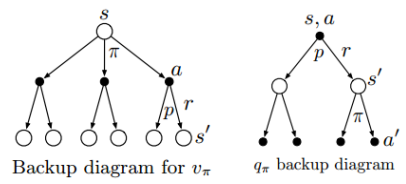
\includegraphics[scale=0.5]{value_functions}
\centering
\caption{Value and State-Value Functions}
\end{figure}

\noindent
\textbf{Optimal State Value Function}
A policy $\pi$ is better or equal to another policy $\pi^{\prime}$ if its
expected return is greater than or equal to that of $\pi^{\prime}$ for all
states ($\pi^{\prime} \geq \pi^{\prime}$ if and only if $v_{\pi}(s) \geq
v_{\pi^{\prime}}(s)$). 

\begin{equation}
v_{*}(s) \doteq \max _{\pi} v_{\pi}(s)
\end{equation}

\noindent
\textbf{Optimal Action Value Function and its relation to $v_{*}$}
. Equation 15 gives the expected return for taking action a in state s and
thereafter following an optimal policy. Comparing with equation 11, $v_{\pi}(s)$
represents the value of a state as the summation of future returns. In equation
15, $v_{*}\left(S_{t+1}\right)$ gives the optimal value of all future states
from the given state and action.

\begin{equation}
\begin{aligned}
q_{*}(s, a) &\doteq \max _{\pi} q_{\pi}(s, a)\\
&= \mathbb{E}\left[R_{t+1}+\gamma v_{*}\left(S_{t+1}\right) | S_{t}=s, A_{t}=a\right]
\end{aligned}
\end{equation}

\noindent
\textbf{Relationship between $q_{*}$ and $v_{*}$}\\
- The value of a state under an optimal policy must equal the expected return
for the best action from that state. \\
- Second last line of equation 16 shows that $G_{t} = R_{t+1} + \gamma
v_{*}(S_{t+1})$ when following $\pi_{*}$. \\
- The last line is the same as equation 17. For finite MDPs, the last line of
equation 16 has a unique solution.\\
- $R_{t+1}$ has nothing to do with policy because the first action was not taken
with policy\\
- $\max$ operator turns equation 16 in to a system of nonlinear equations

\begin{equation}
\begin{aligned}
v_{*}(s) &=\max _{a \in A(s)} q_{*}(s, a)\\
&= \max _{a} q_{*}(s, a)\\
&= \max _{a} \mathbb{E}_{\pi_{*}}[G_{t} | S_{t} = s, A_{t} = a]\\
&= \max _{a} \mathbb{E}[R_{t+1} + \gamma v_{*}(S_{t+1}) | S_{t} = s, A_{t} = a]\\
&= \max _{a} \sum_{s^{\prime}, r} p(s^{\prime}, r | s, a)[r + \gamma v_{*}(s^{\prime})]
\end{aligned}
\end{equation}

\newpage
\noindent
\textbf{Bellman Optimality Equations}\\

\begin{equation}
\begin{aligned}
v_{*}(s) & = \max _{a} \mathbb{E}\left[R_{t+1}+\gamma v_{*}\left(S_{t+1}\right) | S_{t}=s, A_{t}=a\right]\\
&= \max _{a} \sum_{s^{\prime}, r} p\left(s^{\prime}, r | s, a\right)\left[r+\gamma v_{*}\left(s^{\prime}\right)\right]
\end{aligned}
\end{equation}

\begin{equation}
\begin{aligned}
q_{*}(s, a)&=\mathbb{E}\left[R_{t+1}+\gamma \max _{a^{\prime}} q_{*}\left(S_{t+1}, a^{\prime}\right) | S_{t}=s, A_{t}=a\right] \\
&=\sum_{s^{\prime}, r} p\left(s^{\prime}, r | s, a\right)\left[r+\gamma \max _{a^{\prime}} q_{*}\left(s^{\prime}, a^{\prime}\right)\right]
\end{aligned}
\end{equation}

\noindent
In $v_{*}$, the next best action is selected based on the expected reward and
value of future states. In $q_{*}$, the state and action is given as well as the
reward. From the new state $s^{\prime}$, the best action is chosen.

\begin{figure}[h]
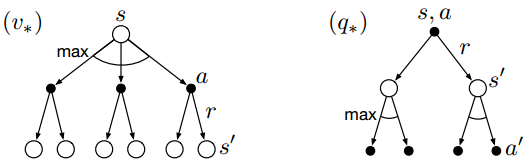
\includegraphics[scale=0.5]{bellman_optimality}
\centering
\caption{Bellman Optimality Equations}
\end{figure}

\noindent
\section{Dynamic Programming}

\noindent
\textbf{Policy Evaluation}\\
- turn Bellman equation from equation 11 in to an update rule\\
- maximum bootstrapping: $v_{k}(s^{\prime})$ is using a previous estimate

\begin{equation}
\begin{aligned}
v_{k+1}(s) & \doteq \mathbb{E}_{\pi}\left[R_{t+1}+\gamma v_{k}\left(S_{t+1}\right) | S_{t}=s\right] \\
&=\sum_{a} \pi(a | s) \sum_{s^{\prime}, r} p\left(s^{\prime}, r | s, a\right)\left[r+\gamma v_{k}\left(s^{\prime}\right)\right]
\end{aligned}
\end{equation}

\noindent
\textbf{Policy Evaluation Steps}\\
- for state in states\\
---- for action in actions available in each state\\
-------- calculate value of state using equation 19 \\
-------- (value = sum all values of each action together for each state (ie. 4
actions in a state = 1 total value))\\
---- replace old value of state with newly calculated value\\
---- calculate the change in value of each state with only the maximum
difference remembered\\
- stop looping if the maximum change in state values falls below a threshold\\

\newpage
\noindent
\textbf{Policy Improvement}\\
- greedy policy = guaranteed to be optimal\\
- one-step greedy lookahead

\begin{equation}
\begin{aligned}
\pi^{\prime}(s) & \doteq \underset{a}{\arg \max } q_{\pi}(s, a) \\
&=\underset{a}{\arg \max } \mathbb{E}\left[R_{t+1}+\gamma v_{\pi}\left(S_{t+1}\right) | S_{t}=s, A_{t}=a\right] \\
&=\underset{a}{\arg \max } \sum_{s^{\prime}, r} p\left(s^{\prime}, r | s, a\right)\left[r+\gamma v_{\pi}\left(s^{\prime}\right)\right]
\end{aligned}
\end{equation}

\noindent
Policy is represented $s \times a$ table where each row represents a state and
each column represents an action. The value within each entry of the table
represent the probability of taking that action, when in that state, using a
probabilistic policy.\\

\noindent
At this stage, there is a value calculated for every state using policy
evaluation already.\\

\noindent
\textbf{Policy Improvement Steps}\\
- for state in states \\
---- choose the best action with the current policy (argmax)\\
---- for action in actions available in each state \\
-------- calculate action values for each action using equation 20 without the
argmax\\
--------(this creates a $1 \times a$ vector where each element is an
action value $q$)\\
---- select the best action in the $ 1 \times a$ vector (equation 20 with
argmax)\\
---- if action chosen with the current policy is not the calculated best
action\\
-------- policy is unstable\\
---- update the policy with the new best action\\

\noindent
\textbf{Policy Iteration}\\
- built on the fundamentals of value iteration\\
- more efficient (CPU time) than value iteration

\begin{figure}[h]
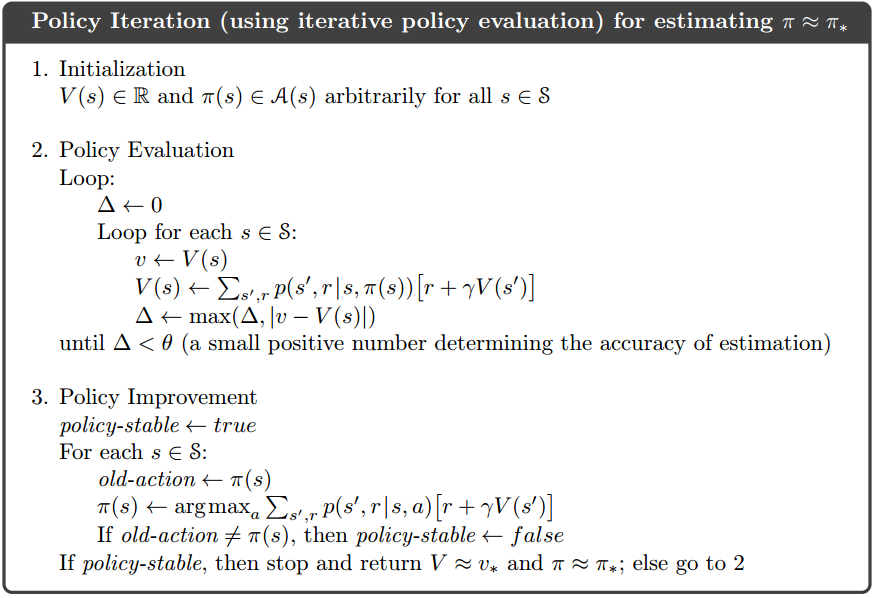
\includegraphics[scale=0.4]{policy_iteration}
\centering
\caption{Policy Iteration}
\end{figure}

\newpage
\noindent
\textbf{Value Evaluation}\\
- Policy iteration is faster because policy converges quicker
than value functions\\
- Bellman Optimality Equation (equation 17) turned in to an update rule \\
- Formally requires infinite number of iterations to converge exactly to $v_{*}$
but we stop before then \\
- Only guarantees $\epsilon - optimality$ (theoretically)\\
- All algorithms converge to an optimal policy for discounted finite MDPs\\
- When $\gamma$ is close to 1, iteration goes forever = making value iteration
inefficient\\
- Policy iteration converges faster even for smaller $\gamma$
- Main difference between Value Iteration and Policy Iteration\\
-- In value iteration, instead of summing values from all actions per state,
take only the best action value per state as the value of that state\\
- Value iteration update is identical to policy evaluation except that the max
is taken over all actions\\

\begin{equation}
\begin{aligned}
v_{k+1}(s) & \doteq \max _{a} \mathbb{E}\left[R_{t+1}+\gamma v_{k}\left(S_{t+1}\right) | S_{t}=s, A_{t}=a\right] \\
&=\max _{a} \sum_{s^{\prime}, r} p\left(s^{\prime}, r | s, a\right)\left[r+\gamma v_{k}\left(s^{\prime}\right)\right]
\end{aligned}
\end{equation}

\noindent
\textbf{Value Iteration Steps}\\
- for state in states \\
---- for action in actions available in each state \\
-------- calculate action values for each action using equation 21 without the
max\\
--------(this creates a $1 \times a$ vector where each element is an
action value $q$)\\
---- value = the best action value in the $ 1 \times a$ vector (equation 21 with
max)\\
---- calculate the change in value of each state with only the maximum
difference remembered\\
- stop looping if the maximum change in state values falls below a threshold\\
- for state in states\\
---- for action in actions available in each state \\
-------- calculate action values for each action using equation 21 without the
max\\
--------(this creates a $1 \times a$ vector where each element is an
action value $q$)\\
---- select the best action in the $ 1 \times a$ vector (equation 21 with
argmax)\\
---- overwrite policy table with best action

\begin{figure}[h]
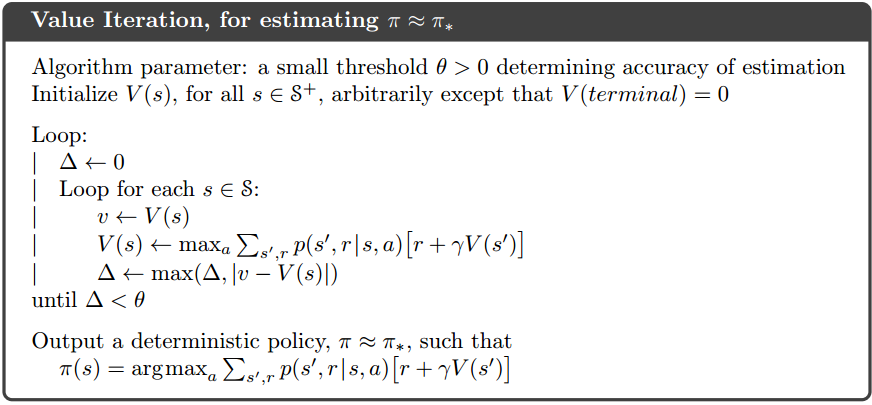
\includegraphics[scale=0.35]{value_iteration}
\centering
\caption{Value Iteration}
\end{figure}

\noindent
\textbf{Summary of Policy and Value Iteration}\\
- Value Iteration: Find optimal value, then extract optimal policy\\
- Policy Iteration: Find value, then extract optimal policy\\

\newpage
\noindent
\section{Monte Carlo Methods}
- Solving RL based on averaging sample returns\\
- Return after taking an action in one state depends on the actions taken in
later states in the same episode\\
- No boot strapping (DP = max bootstrapping)\\
- can be considered as a way to go from $\pi$ to $v$\\

\noindent
\textbf{First-visit MC Method}\\
- average of the returns following first visit to $s$\\
- more popular, samples are independent (faster convergence)\\
- poor sample efficiency\\

\noindent
\textbf{Every-visit MC Method}\\
- averages the returns following all visits to $s$\\
- more natural to function approximation/eligibility traces\\
- possibly statistically unstable\\

\noindent
The following shows first-visit MC methods.

\begin{figure}[h]
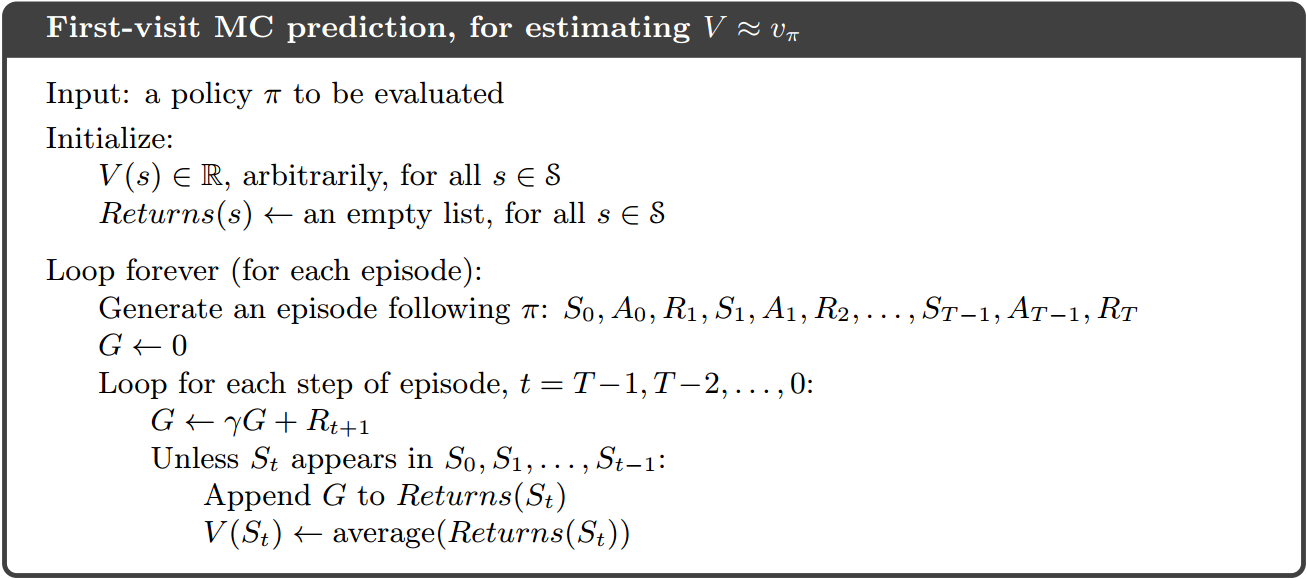
\includegraphics[scale=0.25]{firstvisit_mc}
\centering
\caption{First-visit MC Prediction}
\end{figure}

\noindent
Problem with prior, there will only be one action from each state if following
a deterministic policy. To fix this: \\
- Look at state and action pairs as oppose to just states\\
- Give all state action pair a nonzero probability of being selected (line 6)\\
- Includes a greedy policy at the end to pick the best action in the next
iteration (line 14)\\
- Cons: this solution is unlikely to learn from real experiences but simulated
episodes are fine\\

\begin{figure}[h]
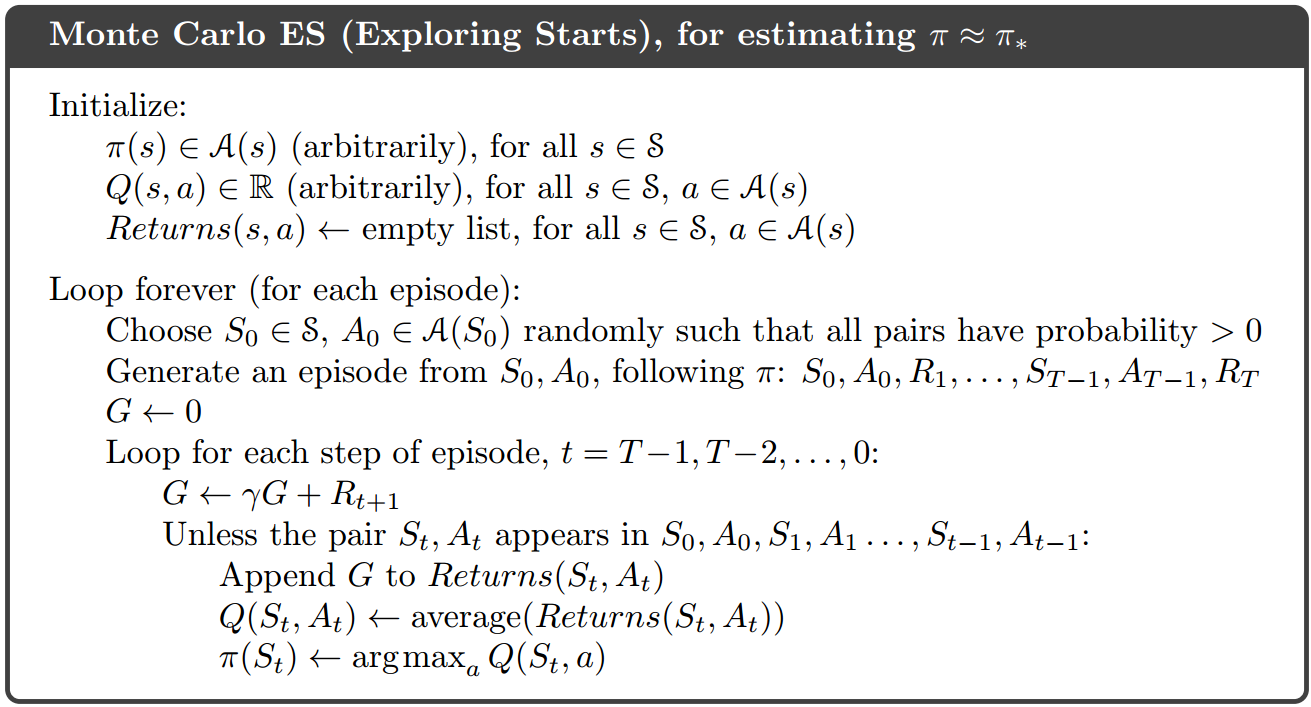
\includegraphics[scale=0.25]{exploringstart_mc}
\centering
\caption{Exploring Start MC Control}
\end{figure}

\newpage
\noindent
\textbf{On-policy vs Off-policy Methods}

\noindent
On-policy methods attempt to evaluate/improve the policy that is used to make
decisions, whereas off-policy methods evaluate/improve a policy different from
that used to generate data. On-policy approach is actually a compromise - it
learns action values not for the optimal policy, but for a near optimal policy
that still explores.\\
- On-policy: unbiased, low bias and variance\\
- Off-policy: biased, high bias and high variance. Slower to converge.\\

\begin{figure}[h]
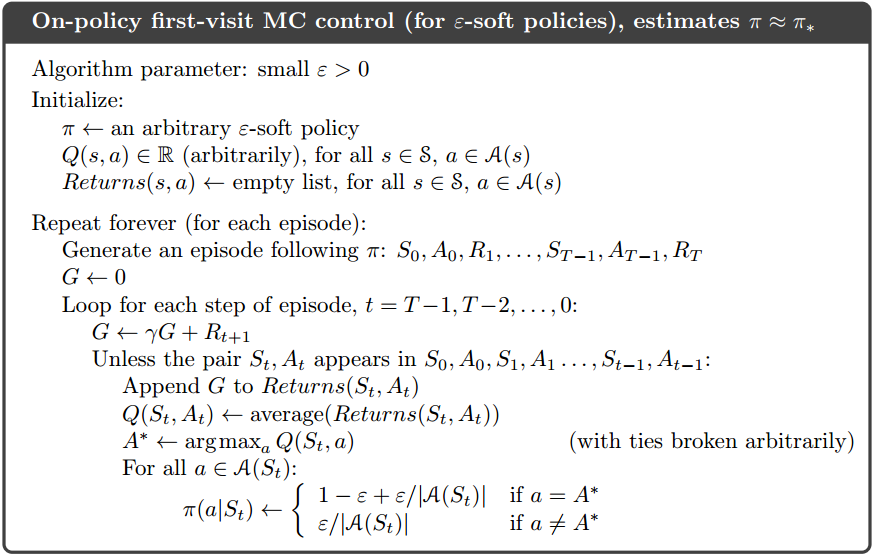
\includegraphics[scale=0.4]{onpolicy_firstvisit_mc}
\centering
\caption{On-policy first-visit MC Control}
\end{figure}

\noindent
\textbf{$\epsilon$ - greedy Exploration}\\
- with probability $\epsilon$, select an action at random\\
- all non-greedy actions are given the minimal probability of selection, $\frac{\varepsilon}{|\mathcal{A}(s)|}$\\
- remaining bulk of probability is given to the greedy action,
$1-\varepsilon+\frac{\varepsilon}{|\mathcal{A}(s)|}$ \\
- the following equation either chooses the greedy action $A^{*}$ or not based on
the probabilities stated

\begin{equation}
\pi\left(a | S_{t}\right) \leftarrow\left\{\begin{array}{ll}
1-\varepsilon+\varepsilon /\left|\mathcal{A}\left(S_{t}\right)\right| & \text { if } a=A^{*} \\
\varepsilon /\left|\mathcal{A}\left(S_{t}\right)\right| & \text { if } a \neq A^{*}
\end{array}\right.
\end{equation}

\noindent
\textbf{Off-policy Evaluation via Importance Sampling}\\
- Target policy: policy being learned about. Becomes deterministic (greedy)
optimal policy.\\
- Behavior policy: policy used to generate behavior. Remains stochastic and more
exploratory.\\

\noindent
\textbf{Importance Sampling Ratio}

\noindent
In order to use episodes from $b$ to estimate values for $\pi$, we require that
every action taken under $\pi$ is also taken, at least occasionally, under $b$.
That is, the following is assumed to be true (known as \textit{coverage}). ISR
eliminates bias from sample so that we can use unbiased samples for learning.

\begin{equation}
\pi(a | s) > 0 \quad \text{implies} \quad b(a|s) > 0
\end{equation}

\noindent
We apply importance sampling to off-policy learning by weighting returns
according to the relative probability of their trajectories occurring under the
target and behavior policies. For example, given a start state $S_{t}$, the
probability of the subsequent state-action trajectory occuring under any policy
$\pi$ is the following. Note, $A_{T}$ will take agent to $S_{T+1}$ which is pass
terminal state.

\begin{equation}
\begin{array}{l}
\operatorname{Pr}\left\{A_{t}, S_{t+1}, A_{t+1}, \ldots, S_{T} | S_{t}, A_{t: T-1} \sim \pi\right\} \\
\quad=\pi\left(A_{t} | S_{t}\right) p\left(S_{t+1} | S_{t}, A_{t}\right) \pi\left(A_{t+1} | S_{t+1}\right) \cdots p\left(S_{T} | S_{T-1}, A_{T-1}\right) \\
\quad=\prod_{k=t}^{T-1} \pi\left(A_{k} | S_{k}\right) p\left(S_{k+1} | S_{k}, A_{k}\right)
\end{array}
\end{equation}

\newpage
\noindent
The relative probability of the trajectory under the target and behavior
policies is shown below. Note, the ratio depends on the policies and not on the
MDP. Note, $\rho_{t: T-1}$ is a scalar value.

\begin{equation}
\rho_{t: T-1} \doteq \frac{\prod_{k=t}^{T-1} \pi\left(A_{k} | S_{k}\right) p\left(S_{k+1} | S_{k}, A_{k}\right)}{\prod_{k=t}^{T-1} b\left(A_{k} | S_{k}\right) p\left(S_{k+1} | S_{k}, A_{k}\right)}=\prod_{k=t}^{T-1} \frac{\pi\left(A_{k} | S_{k}\right)}{b\left(A_{k} | S_{k}\right)}
\end{equation}

\noindent
Convert returns $G_{t}$ due to the behavior policy to expected returns under the
target policy.

\begin{equation}
\mathbb{E}\left[\rho_{t: T-1} G_{t} | S_{t}=s\right]=v_{\pi}(s)
\end{equation}

\noindent
\textbf{Ordinary Importance Sampling}\\
- $\mathcal{T}(s)$ represent the time steps in which state s is visited (norm =
total number of samples)\\
- To estimate $v_{\pi}(s)$, simply scale the returns by the ratios and average
the results\\
- $\left\{G_{t}\right\}_{t \in \mathcal{T}(s)}$ are the returns that pertain to
state $s$ \\
- $\left\{\rho_{t: T(t)-1}\right\}_{t \in \mathcal{T}(s)}$ are the corresponding
ratios\\
- First visit: unbiased, high variance (unbounded)\\
- Every visit: biased
\begin{equation}
V(s) \doteq \frac{\sum_{t \in \mathcal{T}(s)} \rho_{t: T(t)-1} G_{t}}{|\mathcal{T}(s)|}
\end{equation}

\noindent
\textbf{Weighted Importance Sampling}\\
- Weighted average\\
- First visit: biased (though the bias converges asymptotically to zero), variance converges to zero\\
- In practice, this method has dramatically lower variance and is preferred.\\
- Every visit: biased
\begin{equation}
V(s) \doteq \frac{\sum_{t \in \mathcal{T}(s)} \rho_{t: T(t)-1} G_{t}}{\sum_{t \in \mathcal{T}(s)} \rho_{t: T(t)-1}}
\end{equation}

\noindent
\textbf{Comparison of Ordinary and Weighted}

\noindent
If you only have one sample, weighted importance would equal $G_{t}$ as the
ratio in the numerator and denominator cancel out. For ordinary, the denominator
would equal to 1, and the result is equivalent to $\rho_{t: T(t)-1} G_{t}$. If
the ratio was 10, which indicates that the trajectory observed is 10 times as
likely under the target policy as under the behavior policy.\\

\noindent
\textbf{Incremental Implementation: Ordinary Importance Sampling}
\begin{equation}
V_{n}=\frac{\sum_{k=1}^{n-1} W_{k} G_{t}}{n-1}
\end{equation}
\begin{equation}
V_{n+1}=V_{n}+\frac{1}{n}\left(W_{n} G_{n}-V_{n}\right)
\end{equation}

\noindent
\textbf{Incremental Implementation: Weighted Importance Sampling}\\
- $W_{i}=\rho_{t_{i}: T\left(t_{i}\right)-1}$\\
- $G_{1}, G_{2}, \dots, G_{n-1}$\\

\noindent
To estimate the following, 
\begin{equation}
V_{n}=\frac{\sum_{k=1}^{n-1} W_{k} G_{k}}{\sum_{k=1}^{n-1} W_{k}}
\end{equation}

\noindent
Need to keep $V$ up to date as we obtain a single additional return $G_{n}$.

\begin{equation}
V_{n+1}=V_{n}+\frac{W_{n}}{C_{n}}\left[G_{n}-V_{n}\right]
\end{equation}

\noindent
In addition to keeping track of $V_{n}$, must also maintain a cumulative sum of
the weights $C_{n}$ given to the first $n$ returns

\begin{equation}
C_{n+1}=C_{n}+W_{n+1}
\end{equation}

\newpage
\noindent
\textbf{Off-policy MC Prediction}

\noindent
- Off-policy with weighted importance sampling\\ 
- Can be applied to on-policy by choosing the target and behavior policies the
same ($\pi = b$) and $W = 1$ where $W$ is the importance sampling ratio.

\begin{figure}[h]
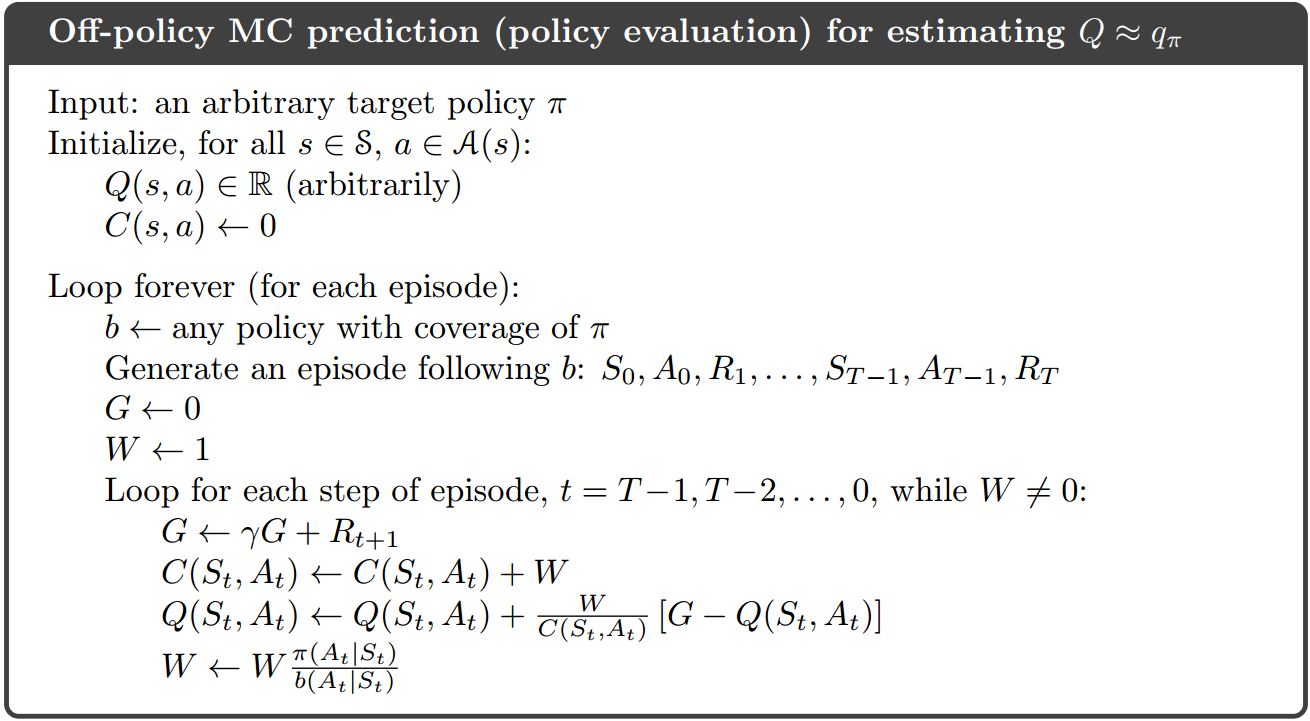
\includegraphics[scale=0.25]{offpolicy_mc_prediction}
\centering
\caption{Off-policy MC Prediction}
\end{figure}

\noindent
\textbf{Off-policy MC Control}

\noindent
What does the last two line of the following pseudo-code mean?

\begin{figure}[h]
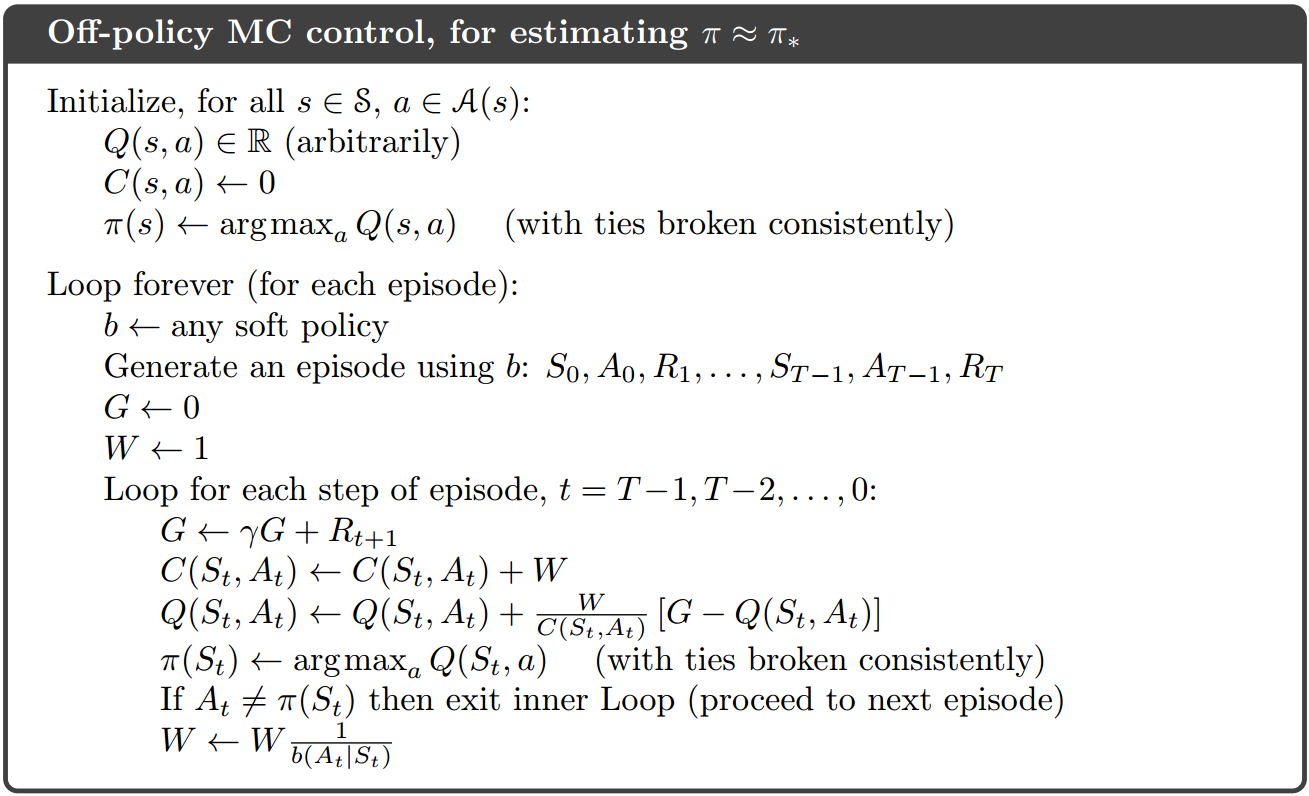
\includegraphics[scale=0.25]{offpolicy_mc_control}
\centering
\caption{Off-policy MC Control}
\end{figure}

\newpage
\noindent
\section{Temporal-Difference Learning}

\noindent
\textbf{TD vs MC}\\

\noindent
TD:\\
- Biased samples because of bootstrapping\\
- Learn after transition: implemented in online - fully incremental fashion\\
- Learn from incomplete episode (used in continuing task)\\
- Sensitive to initial values (initialization of V or Q)\\
- More efficient: in practice, converge faster than MC\\

\noindent
MC:\\
- Solely dependent on environment\\
- No bias, high variance\\
- Learn at the end of episode: delayed learning\\
- Only used with episodic tasks\\
- Insensitive to initial values\\

\noindent
When sample size is finite, may converge to different values.\\

\noindent
\textbf{Monte Carlo (every visit) - Prediction}
: need $G_{t}$ (obtained at the end of the episode) to perform update

\begin{equation}
V\left(S_{t}\right) \leftarrow V\left(S_{t}\right)+\alpha\left[G_{t}-V\left(S_{t}\right)\right]
\end{equation}

\noindent
\textbf{Temporal Difference TD(0) - Prediction}
: need just the next reward $R_{t+1}+\gamma V\left(S_{t+1}\right)$ to perform
update

\begin{equation}
V\left(S_{t}\right) \leftarrow V\left(S_{t}\right)+\alpha\left[R_{t+1}+\gamma V\left(S_{t+1}\right)-V\left(S_{t}\right)\right]
\end{equation}

\noindent
where the TD error is 

\begin{equation}
\delta_{t} \doteq R_{t+1}+\gamma V\left(S_{t+1}\right)-V\left(S_{t}\right)
\end{equation}

\begin{figure}[h]
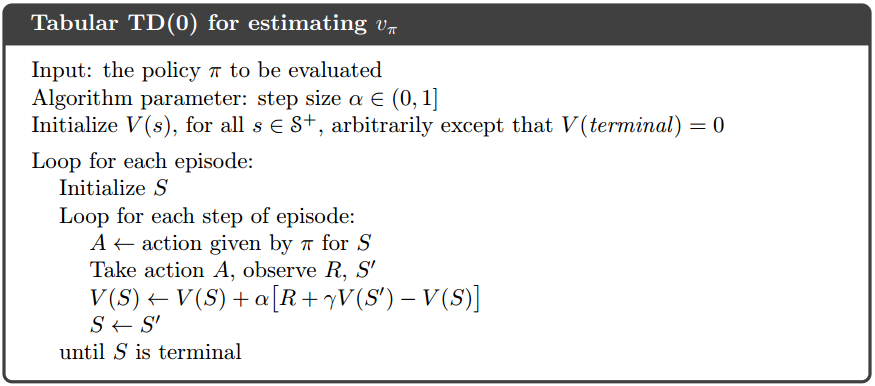
\includegraphics[scale=0.4]{onestep_td}
\centering
\caption{One step TD}
\end{figure}

\noindent
\textbf{SARSA: On-policy TD Control}\\
- Learn an action-value function ($q_{\pi}(s, a)$) rather than a state-value function\\
- Consider transitions from state-action pair to state-action pair, as oppose to
state to state\\

\begin{figure}[h]
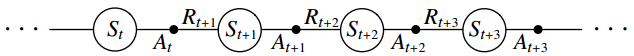
\includegraphics[scale=0.5]{sarsa_diagram}
\centering
\caption{SARSA Diagram}
\end{figure}

\newpage
\noindent
\textbf{SARSA Update}

\begin{equation}
Q\left(S_{t}, A_{t}\right) \leftarrow Q\left(S_{t}, A_{t}\right)+\alpha\left[R_{t+1}+\gamma Q\left(S_{t+1}, A_{t+1}\right)-Q\left(S_{t}, A_{t}\right)\right]
\end{equation}

\noindent
- In the code below, line 8 is where the policy is being optimized (choosing the
next best action based on the state arrived). Note, this code only returns $Q$
and not $Q^{*}$.\\
- On policy because it estimates the return for state action pairs assuming the
current policy continues to be followed. Same policy is used to transition and
also update.

\begin{figure}[h]
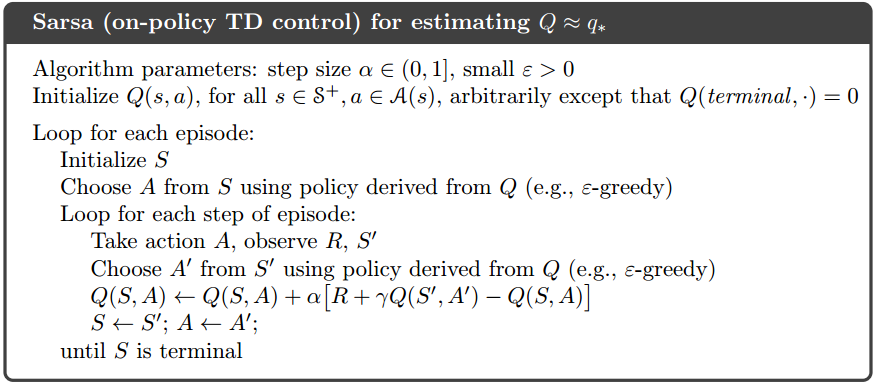
\includegraphics[scale=0.4]{onpolicy_sarsa}
\centering
\caption{SARSA: On-policy TD Control}
\end{figure}

\noindent
\textbf{Q-learning: Off-policy Control}\\
- Instead of choosing $A^{\prime}$ from an $\epsilon-greedy$ policy like in
SARSA, choose the best action with $\max$. \\
- Off policy because Q value is updated using the Q value of the next state and
greedy action. In other words, it estimates the return for $Q(s,a)$ assuming a
greedy policy were followed but is not actually following a greedy policy. One
policy to choose A and another to update Q. If the policy used to choose A is
greedy, the distinction between the two disappears.\\
- Behavior policy is the $\epsilon-greedy$\\
- Convergence is guaranteed under \textit{Robinson-Mouro Condition}

\begin{equation}
Q\left(S_{t}, A_{t}\right) \leftarrow Q\left(S_{t}, A_{t}\right)+\alpha\left[R_{t+1}+\gamma \max _{a} Q\left(S_{t+1}, a\right)-Q\left(S_{t}, A_{t}\right)\right]
\end{equation}

\begin{figure}[h]
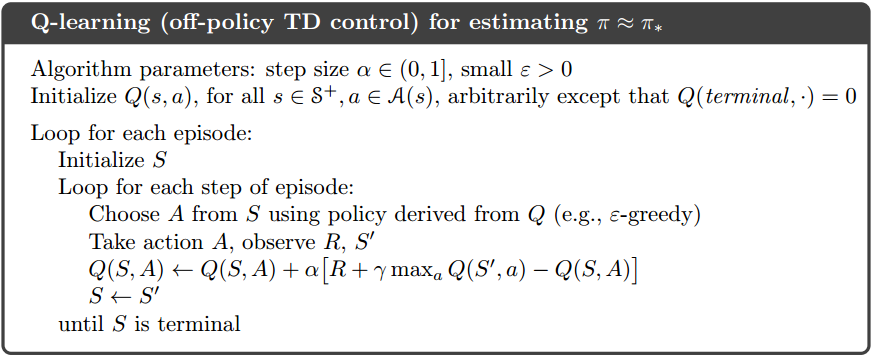
\includegraphics[scale=0.4]{offpolicy_qlearning}
\centering
\caption{Q-learning: Off-policy TD Control}
\end{figure}

\newpage
\noindent
\section{$n$-step Bootstrapping}
- Bootstrapping works best if it is over a length of time in which a significant
and recognizable state change has occurred \\
- Eligibility traces: enable bootstrapping over multiple time intervals
simultaneously \\
- 2 step update = based on the first 2 rewards and the estimated value of teh
state 2 steps later\\

\begin{figure}[h]
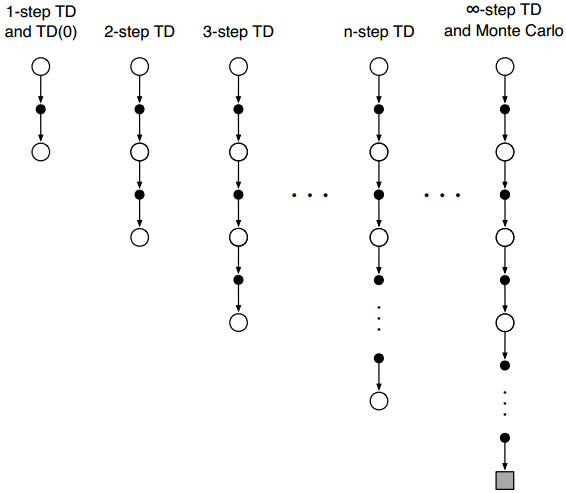
\includegraphics[scale=0.3]{nstep}
\centering
\caption{n-step Methods}
\end{figure}

\noindent
\textbf{Monte Carlo Return}
\begin{equation}
G_{t} \doteq R_{t+1}+\gamma R_{t+2}+\gamma^{2} R_{t+3}+\cdots+\gamma^{T-t-1} R_{T}
\end{equation}

\noindent
\textbf{One Step Return}
\begin{equation}
G_{t: t+1} \doteq R_{t+1}+\gamma V_{t}\left(S_{t+1}\right)
\end{equation}

\noindent
\textbf{Two Step Return}
\begin{equation}
G_{t: t+2} \doteq R_{t+1}+\gamma R_{t+2}+\gamma^{2} V_{t+1}\left(S_{t+2}\right)
\end{equation}

\noindent
\textbf{n-step Return}
\begin{equation}
G_{t: t+n} \doteq R_{t+1}+\gamma R_{t+2}+\cdots+\gamma^{n-1} R_{t+n}+\gamma^{n} V_{t+n-1}\left(S_{t+n}\right)
\end{equation}

\noindent
\textbf{$n$-step TD Prediction}\\
- Line 15: adding up the rewards\\
- Example: $t = 3, n = 2, \tau = 2, G = \sum_{i=3}^{min(4, T)} = R_{3} + \gamma R_{4} + \gamma^{2} V(S_{4})$
\begin{figure}[h]
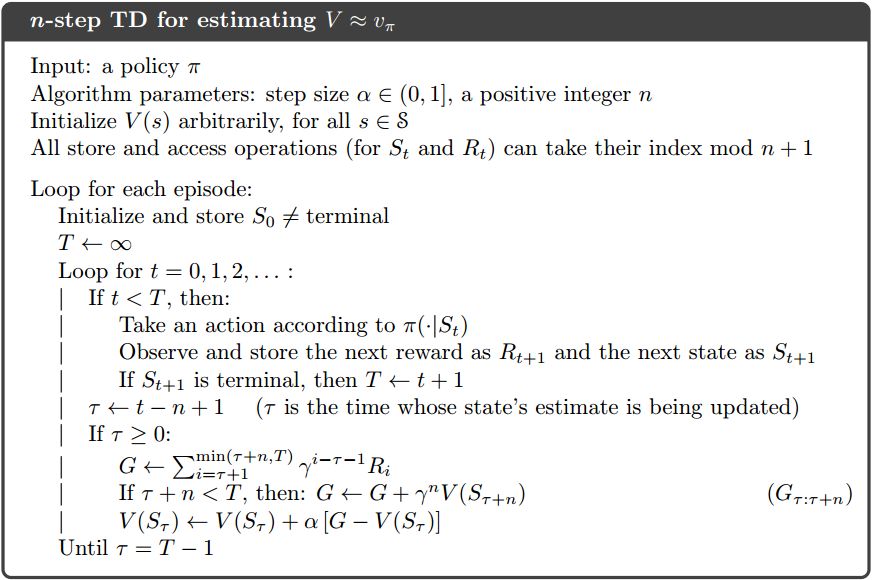
\includegraphics[scale=0.4]{nstep_td}
\centering
\caption{n-step TD Prediction}
\end{figure}

\newpage
\noindent
\textbf{$n$-step SARSA}

\noindent
Switch states for state-action pairs and then use $\epsilon - greedy$ policy.
Given t+1, t+n-1, t+n, what is the time of learning? Should be at time t.

\begin{equation}
G_{t: t+n} \doteq R_{t+1}+\gamma R_{t+2}+\cdots+\gamma^{n-1} R_{t+n}+\gamma^{n} Q_{t+n-1}\left(S_{t+n}, A_{t+n}\right), \quad n \geq 1,0 \leq t<T-n
\end{equation}

\noindent
Similar to equation 37, the following is the update rule for n-step SARSA

\begin{equation}
Q_{t+n}\left(S_{t}, A_{t}\right) \doteq Q_{t+n-1}\left(S_{t}, A_{t}\right)+\alpha\left[G_{t: t+n}-Q_{t+n-1}\left(S_{t}, A_{t}\right)\right], \quad 0 \leq t<T
\end{equation}

\noindent
- $n$-step SARSA = SARARARAR...SA\\
- $\tau < 0$ = means not enough observations (less than $n$ observations)\\
- need at least $n$ samples/steps to begin learning\\
- learning happens from \textbf{if $\tau \geq 0$}

\begin{figure}[h]
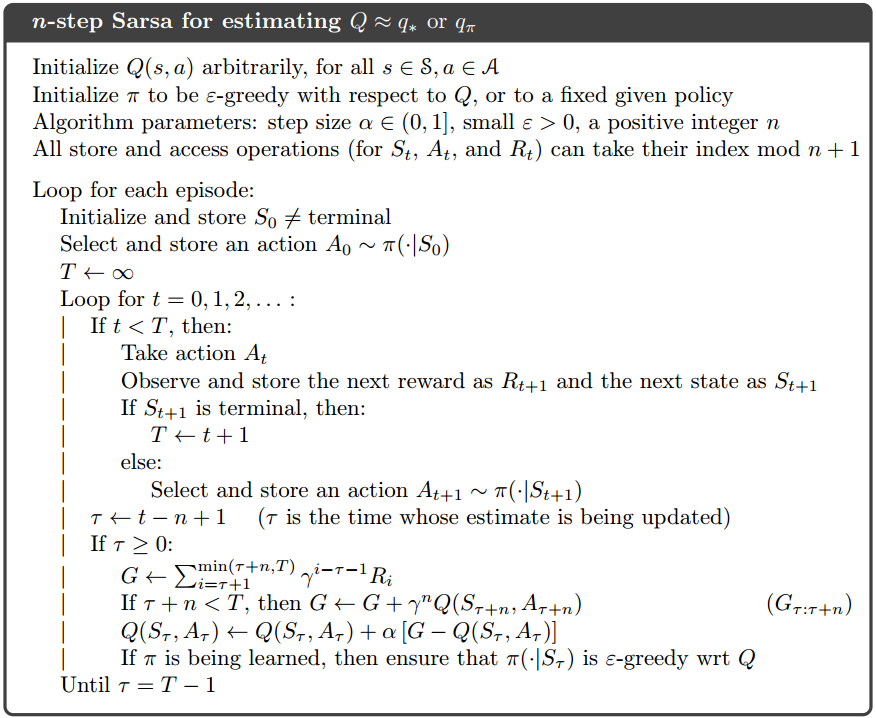
\includegraphics[scale=0.4]{nstep_sarsa}
\centering
\caption{n-step SARSA}
\end{figure}
    
\newpage
\noindent
\textbf{$n$-step Off-policy Learning}

\noindent
\textbf{Off-policy n-step TD}

\noindent
$a_{t}$ is where deviation begins, and $a_{t+n-1}$ is where deviation ends.
$a_{t+n}$ and $s_{t+n}$ are not taken (not used for learning) but they are
needed to calculate $G_{t:t+n}$.

\begin{equation}
V_{t+n}\left(S_{t}\right) \doteq V_{t+n-1}\left(S_{t}\right)+\alpha \rho_{t: t+n-1}\left[G_{t: t+n}-V_{t+n-1}\left(S_{t}\right)\right], \quad 0 \leq t<T
\end{equation}
\begin{figure}[h]
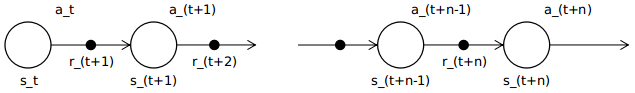
\includegraphics[scale=0.4]{offpolicy_nstep_td_diagram}
\centering
\caption{n-step Off-policy n-step TD}
\end{figure}

\noindent
\textbf{Importance Sampling Ratio}
\begin{equation}
\rho_{t: h} \doteq \prod_{k=t}^{\min (h, T-1)} \frac{\pi\left(A_{k} | S_{k}\right)}{b\left(A_{k} | S_{k}\right)}
\end{equation}

\noindent
\textbf{Off-policy n-step SARSA}

\noindent
Note, the ratio starts and ends one step later than off-policy n-step TD
(equation 45) because the first action $a_{t}$ was given. This is because we are
updating a state-action pair. When updating a value function, the last action is
not taken under policy. When updating a state-action pair, the last action was
taken with behavior policy. In other words, we do not care how likely we were to
select the action; now that we have selected it we want to learn fully from what
happens, with importance sampling only for subsequent actions.
\begin{equation}
Q_{t+n}\left(S_{t}, A_{t}\right) \doteq Q_{t+n-1}\left(S_{t}, A_{t}\right)+\alpha \rho_{t+1: t+n}\left[G_{t: t+n}-Q_{t+n-1}\left(S_{t}, A_{t}\right)\right]
\end{equation}

\noindent
There is a typo in the code below where $\rho$ is calculated. Instead of summing
from $\tau + 1$ to $\tau + n -1$ in line 20, should just be $\tau + n$ as
described in equation 47 (the index shift). The last action is chosen by the
behavior policy and therefore should be included in the importance sampling
ratio's consideration.

One can convert the following code to Q-learning by adding $\max Q(s_{t+n}, a)$
to line 22 like in equation 38. In this case, the previous typo is no longer a
mistake. Normally, in Q-learning, you do not need importance sampling ratio. But
in n-step, there are n-transitions in which importance sampling ratio must be
applied to until the last action which would be chosen by the greedy operator
(behavior policy does not matter for the last action so ISR does not need to be
applied). Additionally, $\rho$ is applied to $G - Q$ instead of just $G$ is
because of the way the incremental implementation works.

\begin{figure}[h]
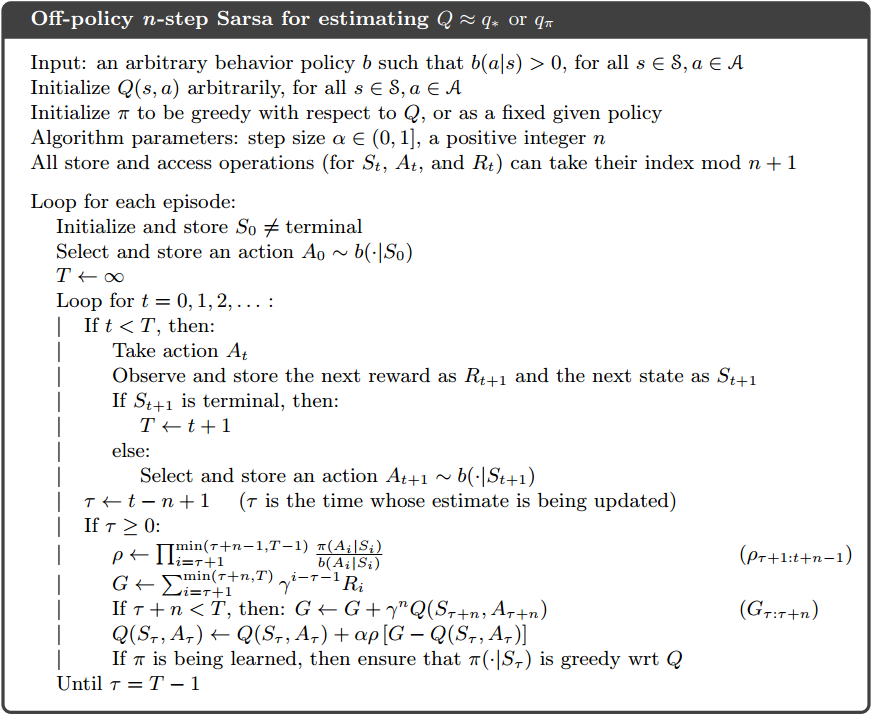
\includegraphics[scale=0.35]{nstep_offpolicy_sarsa}
\centering
\caption{n-step Off-policy SARSA}
\end{figure}

\newpage
\section{Eligibility Trace}


\end{document}
